\documentclass[a4paper,10pt]{report}

\usepackage[english]{babel}

\setcounter{secnumdepth}{4}
\setcounter{tocdepth}{4}
\makeatletter
\newcounter {subsubsubsection}[subsubsection]
\renewcommand\thesubsubsubsection{\thesubsubsection .\@arabic\c@subsubsubsection}
\newcommand\subsubsubsection{\@startsection{subsubsubsection}{4}
    {\z@}%
    {-3.25ex\@plus -1ex \@minus -.2ex}%
    {1.5ex \@plus .2ex}%
    {\normalfont\normalsize\bfseries}
}
\renewcommand\paragraph{\@startsection{paragraph}{5}
    {\z@}%
    {3.25ex \@plus1ex \@minus.2ex}%
    {-1em}%
    {\normalfont\normalsize\bfseries}
}
\renewcommand\subparagraph{\@startsection{subparagraph}{6}
    {\parindent}%
    {3.25ex \@plus1ex \@minus .2ex}%
    {-1em}%
    {\normalfont\normalsize\bfseries}
}
\newcommand*\l@subsubsubsection{\@dottedtocline{4}{10.0em}{4.1em}}
\renewcommand*\l@paragraph{\@dottedtocline{5}{10em}{5em}}
\renewcommand*\l@subparagraph{\@dottedtocline{6}{12em}{6em}}
\newcommand*{\subsubsubsectionmark}[1]{}
\makeatother

\usepackage[colorlinks=true]{hyperref} %http://www.ctan.org/tex-archive/macros/latex/contrib/hyperref/
\hypersetup{urlcolor=black,linkcolor=black}

\makeatletter
\def\toclevel@subsubsubsection{4}
\def\toclevel@paragraph{5}
\def\toclevel@subparagraph{6}
\makeatother

\usepackage[utf8]{inputenc}
\usepackage[T1]{fontenc}
\usepackage[table]{xcolor}
\usepackage{mathpazo} %http://www.ctan.org/tex-archive/fonts/mathpazo
\usepackage{stmaryrd} %http://www.ctan.org/pkg/stmaryrd
\usepackage{amsmath} %http://www.ctan.org/pkg/amsmath
\usepackage{amssymb}
\usepackage{mathrsfs}
\usepackage{boiboites}

\usepackage{amsthm} %http://www.ctan.org/pkg/amsthm
\usepackage{proof}
\usepackage{auto-pst-pdf}

\usepackage{footmisc} %http://www.ctan.org/tex-archive/macros/latex/contrib/footmisc

\usepackage{enumerate}
\usepackage{ulem} %http://www.ctan.org/tex-archive/macros/latex/contrib/ulem
\normalem
\usepackage{cancel} %http://www.ctan.org/tex-archive/macros/latex/contrib/cancel

\usepackage{fullpage} %http://www.ctan.org/tex-archive/macros/latex/contrib/preprint/
\setlength{\parindent}{0pt}
\setlength{\parskip}{\medskipamount}

\renewcommand{\thefootnote}{\fnsymbol{footnote}}

\usepackage{pgffor}
\usepackage{tikz}
\usetikzlibrary{arrows,shapes.arrows, chains, positioning, automata, graphs}
\usepackage{graphviz}

\usepackage[ruled,vlined,english]{algorithm2e}
\providecommand{\SetAlgoLined}{\SetLine}
\providecommand{\DontPrintSemicolon}{\dontprintsemicolon}

\usepackage{forest}
\usepackage{comment} %http://www.ctan.org/tex-archive/macros/latex/contrib/comment
\usepackage{multirow} %http://www.ctan.org/tex-archive/macros/latex/contrib/multirow
\usepackage{diagbox} %http://www.ctan.org/tex-archive/macros/latex/contrib/diagbox

\usepackage{placeins}
\usepackage{wasysym}

\newboxedtheorem[boxcolor=red, background=red!5, titlebackground=red!50,titleboxcolor = black]{theorem}{Theorem}{TheC}
\newboxedtheorem[boxcolor=orange, background=orange!5, titlebackground=orange!50,titleboxcolor = black]{definition}{Definition}{DefC}
\newboxedtheorem[boxcolor=blue, background=blue!5, titlebackground=blue!20,titleboxcolor = black]{proposition}{Proposition}{TheC}
\newboxedtheorem[boxcolor=cyan, background=cyan!5, titlebackground=cyan!20,titleboxcolor = black]{corollary}{Corollary}{TheC}
\newboxedtheorem[boxcolor=black, background=black!0, titlebackground=black!20,titleboxcolor = black]{remark}{Remark}{RemC}
\newboxedtheorem[boxcolor=green!70!black, background=green!70!black!5, titlebackground=green!70!black!30,titleboxcolor = black]{notation}{Notation}{NotC}
\newboxedtheorem[boxcolor=yellow, background=yellow!0, titlebackground=yellow!30,titleboxcolor = black]{example}{Example}{ExeC}
\newboxedtheorem[boxcolor=magenta, background=magenta!5, titlebackground=magenta!30,titleboxcolor = black]{lemma}{Lemma}{TheC}
\newboxedtheorem[boxcolor=magenta, background=magenta!5, titlebackground=magenta!30,titleboxcolor = black]{fact}{Fact}{TheC}
\newboxedtheorem[boxcolor=cyan, background=cyan!5, titlebackground=cyan!20,titleboxcolor = black]{consequence}{Consequence}{TheC}
\newboxedtheorem[boxcolor=black, background=black!0, titlebackground=black!20,titleboxcolor = black]{algo}{Algorithm}{AlgoC}
\newboxedtheorem[boxcolor=black, background=black!0, titlebackground=black!20,titleboxcolor = black]{conjecture}{Conjecture}{ConjC}

\newcommand{\RR}{\mathbb{R}}
\newcommand{\QQ}{\mathbb{Q}}
\newcommand{\CC}{\mathbb{C}}
\newcommand{\ZZ}{\mathbb{Z}}
\newcommand{\NN}{\mathbb{N}}
\newcommand{\GG}{\mathbb{G}}
\newcommand{\PP}{\mathbb{P}}
\newcommand{\EE}{\mathbb{E}}
\newcommand{\KK}{\mathbb{K}}
\newcommand{\IE}{\mathbb{E}}
\newcommand{\IR}{\mathbb{R}}
\newcommand{\IZ}{\mathbb{Z}}
\newcommand{\IN}{\mathbb{N}}
\newcommand{\IP}{\mathbb{P}}
\newcommand{\IF}{\mathbb{F}}

\newcommand{\cF}{\mathcal{F}}
\newcommand{\ck}{\mathcal{K}}
\newcommand{\cK}{\mathcal{K}}
\newcommand{\cL}{\mathcal{L}}
\newcommand{\cN}{\mathcal{N}}
\newcommand{\cNU}{\mathcal{NU}}
\newcommand{\cP}{\mathcal{P}}
\newcommand{\A}{\mathcal{A}}
\newcommand{\B}{\mathcal{B}}
\newcommand{\C}{\mathcal{C}}
\newcommand{\E}{\mathcal{E}}
\newcommand{\F}{\mathcal{F}}
\newcommand{\G}{\mathcal{G}}
\newcommand{\I}{\mathcal{I}}
\newcommand{\K}{\mathcal{K}}
\renewcommand{\L}{\mathcal{L}}
\newcommand{\M}{\mathcal{M}}
\newcommand{\N}{\mathcal{N}}
\newcommand{\R}{\mathcal{R}}
\renewcommand{\S}{\mathcal{S}}
\newcommand{\T}{\mathcal{T}}
\newcommand{\U}{\mathcal{U}}
\newcommand{\V}{\mathcal{V}}
\newcommand{\W}{\mathcal{W}}
\newcommand{\X}{\mathcal{X}}

\newcommand{\bA}{\mathbf{A}}
\newcommand{\bE}{\mathbf{E}}
\newcommand{\bF}{\mathbf{F}}
\newcommand{\bG}{\mathbf{G}}
\newcommand{\bN}{\mathbf{N}}
\newcommand{\bU}{\mathbf{U}}
\newcommand{\bX}{\mathbf{X}}

\newcommand{\ens}[1]{\left\{ #1 \right\}}
\newcommand{\set}[1]{\left\{ #1 \right\}}
\renewcommand{\leq}{\leqslant}
\renewcommand{\geq}{\geqslant}
\renewcommand{\le}{\leqslant}
\renewcommand{\ge}{\geqslant}
\newcommand{\cplx}[1]{\mathcal O \left( #1 \right)}
\newcommand{\floor}[1]{\left \lfloor #1 \right \rfloor}
\newcommand{\ceil}[1]{\left\lceil #1 \right\rceil}
\newcommand{\brackets}[1]{\left\llbracket #1 \right\rrbracket}
\renewcommand{\angle}[1]{\left\langle #1 \right\rangle}
\newcommand{\donne}{\rightarrow}
\newcommand{\gives}{\rightarrow}
\newcommand{\dans}{\to}
\newcommand{\booleen}{\set{0,1}^*}
\newcommand{\eps}{\varepsilon}
\renewcommand{\implies}{~\Rightarrow~}
\newcommand{\tildarrow}{\rightsquigarrow}
\newcommand{\blank}{\texttt{\char32}}
\newcommand{\trans}[1]{\xrightarrow{#1}}
\newcommand{\rules}[1]{\xrightarrow{#1}}
\newcommand{\todo}[1]{\Large\textcolor{red}{#1}\normalsize}
\newcommand{\wtf}[1]{\Large\textcolor{red}{WTF ?! #1}\normalsize}
\newcommand{\argmin}{\text{argmin}}
\newcommand{\rainbowdash}{\vdash}
\newcommand{\notrainbowdash}{\nvdash}
\newcommand{\rainbowDash}{\vDash}
\newcommand{\notrainbowDash}{\nvDash}
\newcommand{\Rainbowdash}{\Vdash}
\newcommand{\notRainbowdash}{\nVdash}
\newcommand{\bottom}{\bot}
\newcommand{\ra}{\rightarrow}
\newcommand{\Ra}{\Rightarrow}
\newcommand{\longra}{\longrightarrow}
\newcommand{\longRa}{\Longrightarrow}
\newcommand{\la}{\leftarrow}
\newcommand{\La}{\Leftarrow}
\newcommand{\longla}{\longleftarrow}
\newcommand{\longLa}{\Longleftarrow}
\newcommand{\lra}{\leftrightarrow}
\newcommand{\LRa}{\Leftrightarrow}
\newcommand{\longlra}{\longleftrightarrow}
\newcommand{\longLRa}{\Longleftrightarrow}
\newcommand{\opname}[1]{\operatorname{#1}}
\newcommand{\suml}{\sum\limits}
\newcommand{\prodl}{\prod\limits}
\newcommand{\liml}{\lim\limits}
\newcommand{\supl}{\sup\limits}
\newcommand{\infl}{\inf\limits}
\newcommand{\maxl}{\max\limits}
\newcommand{\minl}{\min\limits}
\newcommand{\bigcapl}{\bigcap\limits}
\newcommand{\bigcupl}{\bigcup\limits}


%Optim
\newcommand{\Det}{\operatorname{Det}}
\newcommand{\TU}{\mathcal{TU}}

%Verif
\newcommand{\ifb}{\mathbf{\ if \ }}
\newcommand{\thenb}{\mathbf{\ then \ }}
\newcommand{\elseb}{\mathbf{\ else \ }}
\newcommand{\dob}{\mathbf{\ do \ }}
\newcommand{\whileb}{\mathbf{\ while \ }}
\newcommand{\abortb}{\mathbf{\ abort \ }}
\newcommand{\skipb}{\mathbf{\ skip \ }}
\newcommand{\inb}{\mathbf{\ in \ }}
\newcommand{\withb}{\mathbf{\ with \ }}
\newcommand{\raiseb}{\mathbf{\ raise \ }}
\newcommand{\trapb}{\mathbf{\ trap \ }}

%CalcForm
\newcommand{\DFT}{\operatorname{DFT}}
\newcommand{\val}{\operatorname{val}}
\newcommand{\Ker}{\operatorname{Ker}}
\newcommand{\pgcd}{\operatorname{pgcd}}
\newcommand{\Tr}{\operatorname{Tr}}

%Compil
\def\changemargin#1#2{\list{}{\rightmargin#2\leftmargin#1}\item[]}
\let\endchangemargin=\endlist

%AlgoPar
\newcommand{\forto}{\text{\bf\ to\ }}


%EvalPerf
\newcommand{\Var}[1]{\text{Var}\left( #1 \right)}
\newcommand{\prob}[1]{\PP\left( #1 \right)}
\newcommand{\esp}[1]{\EE\left[ #1 \right]}
\newcommand{\dd}{\mathrm{d}}


%SystDist
\newcommand{\Receive}{\texttt{Receive~}}
\newcommand{\Send}{\texttt{Send~}}


%Preuves
\newcommand{\betaeq}{=_\beta}
\newcommand{\betared}{\vartriangleright_\beta}
\newcommand{\parabetared}{\vartriangleright_{||\beta}}
\newcommand{\Ackermann}{\A}
\newcommand{\Ter}{\mathcal{T}er}


%Cplx
\newcommand{\Time}{\textsc{Time}}
\newcommand{\TIME}{\textsc{Time}}

\newcommand{\dtime}{\textsc{DTime}}
\newcommand{\dTime}{\textsc{DTime}}
\newcommand{\DTime}{\textsc{DTime}}

\newcommand{\ntime}{\textsc{NTime}}
\newcommand{\nTime}{\textsc{NTime}}
\newcommand{\NTime}{\textsc{NTime}}

\renewcommand{\P}{\textsc{P}}
\newcommand{\coP}{co\text{-}\textsc{P}}

\newcommand{\pTime}{\textsc{PTime}}
\newcommand{\PTime}{\textsc{PTime}}

\newcommand{\NP}{\textsc{NP}}

\newcommand{\npTime}{\textsc{NPTime}}
\newcommand{\NPTime}{\textsc{NPTime}}

\newcommand{\EXP}{\textsc{Exp}}
\newcommand{\expTime}{\textsc{Exp}}
\newcommand{\ExpTime}{\textsc{Exp}}
\newcommand{\EXPTime}{\textsc{Exp}}

\newcommand{\Space}{\textsc{Space}}

\newcommand{\dSpace}{\textsc{DSpace}}
\newcommand{\DSpace}{\textsc{DSpace}}


\newcommand{\nSpace}{\textsc{NSpace}}\newcommand{\NSpace}{\textsc{NSpace}}

\newcommand{\pSpace}{\textsc{PSpace}}
\newcommand{\PSpace}{\textsc{PSpace}}

\newcommand{\npSpace}{\textsc{NPSpace}}
\newcommand{\NpSpace}{\textsc{NPSpace}}
\newcommand{\NPSpace}{\textsc{NPSpace}}

\newcommand{\SpaceTM}{\textsc{SpaceTM}}

\newcommand{\nL}{\textsc{NL}}
\newcommand{\NL}{\textsc{NL}}

\newcommand{\LL}{\textsc{L}}

\newcommand{\coNP}{co\text{-}\textsc{NP}}

\newcommand{\conL}{co\text{-}\textsc{NL}}
\newcommand{\coNL}{co\text{-}\textsc{NL}}

\newcommand{\npc}{\text{\textit{NP-C}}}

\newcommand{\PH}{\textsc{PH}}

\newcommand{\TISP}{\textsc{TISP}}

\newcommand{\Ppoly}{P_{/poly}}

\newcommand{\BPP}{\textsc{BPP}}
\newcommand{\RP}{\textsc{RP}}
\newcommand{\ZPP}{\textsc{ZPP}}
\newcommand{\coBPP}{co\text{-}\textsc{BPP}}
\newcommand{\coRP}{co\text{-}\textsc{RP}}
\newcommand{\coZPP}{co\text{-}\textsc{ZPP}}
\newcommand{\MA}{\textsc{MA}}

\newcommand{\Size}{\textsc{Size}}
\newcommand{\SIZE}{\textsc{Size}}

\newcommand{\dIP}{\mathrm{d}\textsc{IP}}


\newcommand{\vol}{\opname{vol}}
\newcommand{\sgn}{\opname{sgn}}

\title{Analytic Methods in Algorithms and Complexity}
\author{Nisheeth \textsc{Vidhnoi}}
\date{2015-2016}

\begin{document}
\maketitle
\tableofcontents

\newpage

Website: \url{http://theory.epfl.ch/cs435/Home.html}

\chapter*{Introduction and generalities}
    Continuous algorithms techniques to design algorithms for discrete problems.

For example, a graph $G=(V,E)$  is a discrete object: this is a discrete input. With such an input, we can find cuts, flows\dots which are discrete output.

We will interest in function $\RR^n \ra \RR$. We assume that the functions are differentiable (multiple times).


    
\chapter{Convexity and Gradient Descent}
    \section{Definitions}
        The first derivative is the gradient:
\[
    \nabla f = \left( \frac{\partial f}{\partial x_1},\ldots, \frac{\partial f}{\partial x_n} \right)
\]

The second derivative is the Hessian:
\[
    \nabla^2 f = \left(\frac{\partial f}{\partial x_i\partial x_j} \right)_{\substack{i\in\llbracket 1;n\rrbracket\\ j\in\llbracket 1;n\rrbracket}} \in \M_n(\RR^n \to \RR)
\]


\begin{notation}
    For $M\in\M_n(\RR)$ and $(l,L)\in\RR^2$. We note
    \[
        lI_n  \preccurlyeq M \preccurlyeq LI_n
    \]
    if all eigenvalues of $M$ are in $[l;L]$.
\end{notation}

\begin{definition}
    \[
        \forall (x,y) \in {\RR^n}^2, \langle x, y\rangle = \sum\limits_{i=1}^n x_i y_i = x^Ty
    \]
    
    \[
        \lVert x \rVert := \sqrt{\angle{x,x}}
    \]
\end{definition}

\begin{theorem}[\textsc{Cauchy-Schwarz} inequality]
    \[
        \angle{x,y} = \lVert x \rVert \lVert y \rVert
    \]
\end{theorem}

\begin{theorem}[Taylor Expansion]
    $f : \RR^n\to\RR$
    
    \[
        f(y) = f(x) + \angle{\nabla f(x),y-x)} + \frac{1}{2}(y-x)^T \nabla^2 f(x)(y-x) + \ldots
    \]
\end{theorem}

\begin{definition}[Convex set]
    A set $K\subseteq \RR^n$ is convex if
    \[
        \forall (x,y) \in K^2, \forall t\in[0;1], tx+(1-t)y \in K
    \]
\end{definition}

\begin{definition}[Convex function]
    A function $f : \RR^n \to \RR$ is convex if
    \[
        \forall (x,y) \in K^2, \forall t\in[0;1], f(tx+(1-t)y) \leqslant tf(x) + (1-t)f(y)
    \]
\end{definition}

\begin{proposition}
    A function $f$ is convex if and only if
    \[
        f(y) \geqslant f(x) + \angle{\nabla f(x),y-x)}    
    \]
\end{proposition}

\begin{proposition}
    A function $f$ is convex if and only if
    \[
        \forall x\in K, \nabla^2 f(x) \succcurlyeq 0
    \]
\end{proposition}

    \section{Convex optimization}
        \[
    \inf\limits_{x\in K} f(x)
\]

\begin{example}
    Input: $A \in \M_n(\RR)$, $A\geqslant 0$, $b\in\RR^n$.
    
    Goal: Solve $Ax=b$.
    
    $f(x)$ is convex such that $x=\inf\limits_{t} f(t) \Ra A^{-1} b = x$.
    
    $f(x) = \lVert Ax-b \rVert^2 \geqslant 0$
    
    \[
        \begin{aligned}
            \angle{Ax-b, Ax-b} &= x^T A^2x\\
            \nabla^2 f &= A^2
        \end{aligned}
    \]
\end{example}

\begin{example}[Linear programming]
    Input: $A \in \M_{m,n}(\RR)$, $b\in\RR^n$, $c\in\RR^m$.
    
    Goal: $\min\limits \angle{c,x}$ such that $Ax=b$ and $x\geqslant 0$.
\end{example}

\begin{proposition}
    $x$ is optimal iff $\nabla^2f(x) = 0$.
\end{proposition}


        
    \section{Solving Convex Programs (Gradient Descent)}
        Template:
\begin{enumerate}
    \item $i=1$
    \item Starting point $x_i$
    \item Compute $\nabla f(x_i)$.
    \item Either $\nabla f(x_i) = 0$ (OK) or figure out $x_{i+1}$ goto 2.
\end{enumerate}

We don't expect to solve the convex program exactly.

Given $\varepsilon > 0$, the goal is to output a point $x$ such that
\[
    \begin{aligned}
	    f(x^*) &\leqslant f(x)  + \varepsilon\\
	    \lvert f(x)-f(x^*)\rvert &\leqslant \varepsilon
    \end{aligned}
\]

The running time depend of $\frac{1}{\varepsilon}$.


Start with $x_1$.

\[
    x_{t+1} = x_t - \underbrace{\eta_t}_{\substack{>0\\\text{step size}}} \nabla f(x_t)
\]

Why is this algorithm good?


\begin{theorem}
    If $f$ is convex, differentiable, $\nabla f$ is $L$-Lipschitz start at $x_1$ such that $\left\lVert x_1-x^* \right\rVert \leqslant D$, is we pick $T = o\left( \frac{LD^2}{\varepsilon} \right)$, $f(x_T) \leqslant f(x^*) + \varepsilon$.
\end{theorem}

We are allows to change $f$ at time $t$. $f_t$ is convex and $\forall t, \forall x, \lVert \nabla f_t(x) \rVert \leqslant G$.

\begin{corollary}
    If $f_1, f_2,\ldots$, convex differentiable function, $\lVert \nabla f_t\rVert \leqslant G$, then given $\varepsilon > 0$, "good" $x_1$, then after $T \approx \left( \frac{G}{\varepsilon} \right)^2$ iterations, 
    \[
        \underbrace{\frac{1}{T} \sum\limits_{t=1}^T f_t(x_t)}_{\text{algo output}} \leqslant \underbrace{\inf\limits_x \sum_{t=1}^T f_t(x)}_{\text{Best possible}} + \varepsilon
    \]
\end{corollary}

Online convex optimization.


    $\lVert \nabla f \rVert_2 \leqslant \sqrt{n}\lVert \nabla f\rVert_\infty$ So we can use $\lVert\quad\rVert_\infty$\footnote{En dimension finie, toutes les normes sont équivalentes}.



        
\chapter{Multiplicative Weights Update Method}
     
$E_1, \ldots, E_n$ experts. Each expert decide $+1$ or $-1$.
    
\begin{tabular}{c|c|c|c}
    &$E_1$ & $\cdots$ & $E_n$\\
    \hline
    &$\vdots$&&$\vdots$\\
    \hline
    $t$ & $+1$ & $\cdots$ & $-1$
\end{tabular}

Consider majority vote

\[
    \begin{aligned}
        m_i^t &= \# \text{ of mistakes made by }E_i\text{ until }t\\
        M^t &= \#\text{ of mistakes mabe by us}
    \end{aligned}
\]

After your prediction get to see the real answer.

How to measure our performance?

$\frac{M^t}{t}$, $\boxed{M^t- \min\limits_i m_i^t}$

Suppose $E_1, \ldots, E_n$ collude and $> \frac{1}{2}$ of them always output the opposite of the truth (they know). REALLY BAD!

\begin{figure}[!ht]
    \centering
    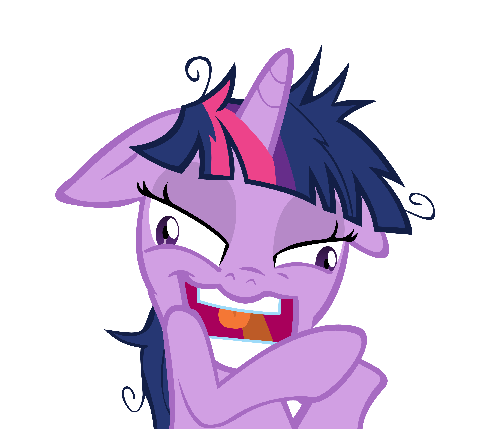
\includegraphics[scale=0.5]{figures/twilight_is_crazy_by_ajdispirito-d52zjfp}
    \caption{This expert want to see you fail}
\end{figure}

\FloatBarrier

$w_i^t \geqslant 0$

Start with $\forall i, w_i^t = 1$.

Weighted majority:
\[
    \sum\limits_{i \text{ votes }+1} w_i^t \ ? \ \sum\limits_{i \text{ votes }-1} w_i^t
\]

How to update weights?

\[
    w_i^t = w_i^t(1-\varepsilon f_i^t)
\]

$f_i^t = [E \text{ is wrong at }t]\footnotemark$\footnotetext{\url{https://en.wikipedia.org/wiki/Iverson_bracket}}

$0 < \varepsilon \leqslant \frac{1}{2}$.

\begin{definition}[Potential]
    \[
        \begin{aligned}
            \Phi^t &= \sum\limits_{i=1}^n w_i^t\\
            \Phi^1 &= n
        \end{aligned}
    \]
\end{definition}

$\Phi^{t+1} \leqslant \Phi^t (?)$

If we don't make a mistake at $t$ does not have to decrease.

Let $t$ such that we made a mistake.

\[
    \begin{aligned}
        \Phi^{t+1} &\leqslant \underbrace{\hspace{10pt}}_{\text{wrong}} + \overbrace{\underbrace{\sum\limits_i w_i^t}_{\text{right}}}^{=\theta}\\
        &= \left( \Phi^t -\theta \right) \left( 1-\varepsilon \right) + \theta\\
        &= \Phi^t(1-\varepsilon) + \theta\varepsilon\\
        &\leqslant \Phi^t(1-\varepsilon) + \frac{\Phi^t}{2}\varepsilon\\
        &= \Phi^t \left( 1- \frac{\varepsilon}{2}\right)
    \end{aligned}
\]
Thus
\[
    \Phi^{t+1} \leqslant \Phi^t\left(1-\frac{\varepsilon}{2}\right)
\]

\[
    \begin{aligned}
        \Phi^{t+1} &\leqslant \Phi^1\left( 1-\frac{\varepsilon}{2}\right)^{M^t}\\
        &= n\left( 1-\frac{\varepsilon}{2}\right)^{M^t}\\
        &\leqslant n e^{-\frac{\varepsilon}{2}M^t}
    \end{aligned}
\]

\[
    \begin{aligned}
        \Phi^{t+1} &= \sum\limits_{i=1}^n w_i^{t+1}\\
        &\overset{\forall i}{\geqslant} w_i^{t+1}\\
        &=(1-\varepsilon)^{m_i^t}\\
        &\overset{?}{=} e^{-\varepsilon m_i^t}
    \end{aligned}
\]

Combining the two last results

\[
    \boxed{\forall i, M^t \leqslant 2 m_i^t + \frac{2\ln n}{\varepsilon}}
\]

\[
    \boxed{t \geqslant \frac{2\ln n}{\varepsilon^2}}
\]

\begin{theorem}
    If we run the WMA, then after $T= \frac{2\ln n}{\varepsilon^2}$,
    \[
        \forall i, \frac{1}{T} M^T \leqslant \frac{2m_i^T}{T} \left( 1+\varepsilon\right) + \varepsilon
    \]
\end{theorem}

$f_i^t$ loss functions.

$f_i^t \in [-1,1]$.

Our strategy at time $t$

$p^t \in \Delta_n$

\[
    \Delta_n = \set{x \vert x \geqslant 0, \sum\limits_{i=1}^n x_i = 1}
\]

Use $p^t$ to make a prediction. Consider $\angle{p^t, f^t}$ loss, $f^t = (f_i^t)^n_{i=1}$.

Pick $i \la p^t$. Output the prediction of $i^\text{th}$  expert.

$\angle{p^t, f^t} = $ probability of making a mistake.

Game : 
\begin{tabular}{ccc}
    You & & Adversary\\
    $p^t \in \Delta_n$ & & \\
    & $\ra$ & \\
    & & $f^t$, $\lVert f^t \rvert_\infty \leqslant 1$\\
    & $\la$ & \\
\end{tabular}

Your loss: $\angle{f^t, p^t}$.

Goal: Find a strategy such that 
\[
    \underbrace{\sum\limits_t \angle{f^t, p^t}}_{\text{your loss}} \leqslant \underbrace{\min_p \angle{f^t, p}}_{\text{Best loss}} + \underbrace{}_{\text{error}}
\]

\bigskip

Algorithm:

$\forall i, w_i^1 = 1$, $p^1 = \frac{w^1}{\Phi^1}$.

$w_i^{t+1} = w_i^t\left( 1-\varepsilon f_i^t\right)$

$p^{t+1} = \frac{w^{t+1}}{\Phi^{t+1}}$ (normalization).

$\left( \Phi^t = \sum\limits_{i=1}^n w_i^t \right)$

\bigskip

Potential function: $\Phi^t= \sum\limits_{i=1}^n w_i^t$.

\begin{enumerate}
    \item $\Phi^{t+1} \leqslant \Phi^t \left( \quad \right)$
        \[
            \begin{aligned}
                \Phi^{t+1} &= \sum\limits_{i=1}^nw_i^{t+1}\\
                &= \sum\limits_{i=1}^nw_i^t\left( 1-\varepsilon f_i^t \right)\\
                &= \sum\limits_{i=1}^nw_i^t- \sum\limits_{i=1}^nw_i^t \varepsilon f_i^t\\
                &\leqslant \Phi^1 e^{-\varepsilon \sum\limits_{j=1}^t \angle{f^i, p^j}}\\
            \end{aligned}       
        \]
    \item $\Phi^{t+1} = \sum\limits_{i=1}^n w_i^{t+1} \overset{\forall i}{\geqslant} w_i^{t+1}$
        \[
            \begin{aligned}
                w_i^{t+1} &= \prod\limits_{j=1}^t \left( 1-\varepsilon f_i^j\right)\\
                &\geqslant \prod\limits_{j=1}^t e^{-\varepsilon f_i^j - \varepsilon ^2(f_i^j)^2}\\
                \Phi^{t+1} &\geqslant e^{-\sum\limits_{j=1}^t \varepsilon f_i^j - \varepsilon^2 \sum\limits_{j=1}^t (f_i^j)^2}
            \end{aligned}
        \]
\end{enumerate}

\[
    e^{-\sum\limits_{j=1}^t \varepsilon f_i^j - \varepsilon^2 \sum\limits_{j=1}^t (f_i^j)^2}\leqslant \Phi^{t+1}\leqslant n e^{-\varepsilon \sum\limits_{j=1}^t \angle{f^i, p^j}}
\]

$\Ra$

\[
    -\sum\limits_{j=1}^t \varepsilon f_i^j - \varepsilon^2 \sum\limits_{j=1}^t (f_i^j)^2 \leqslant \ln n -\varepsilon \sum\limits_{j=1}^t \angle{f^i, p^j}
\]

If we forget $- \varepsilon^2 \sum\limits_{j=1}^t (f_i^j)^2$, we have
\[
    \begin{aligned}
        \text{our loss} &\leqslant \text{loss of }E_i + \frac{\ln n}{\varepsilon}\\
        &\leqslant\sum\limits_{j=1}^t \angle{f^j, p} + \frac{\ln n}{\varepsilon}
    \end{aligned}
\]

How to use MWU? 

Simple:

labelled data $(a_1,l_1), \ldots ,(a_n,l_n)$\dots, labels $\in \set{-1,1}$, $a_i \in \RR^d$ feature vectors.

Goal: find $x$ such that
\[
    \opname{sign}(\angle{x, a_i}) = l_i
\]
$x \geqslant 0$, $\sum\limits_{i=1}^n x_i = 1$

Want $x \in \Delta_n$ such that $\opname{sign}(\angle{x, a_i}) = l_i$ By multiplying $a_i l_i$, we may assume $l_i = 1$.

Problem: find $x\in\Delta_n$ such that $\forall i, \angle{a_i,x} \geqslant 0$. Linear programming\footnote{\url{http://builds.progval.net/ens/cours-m1/Optimisation/Optimisation.pdf}}!

Assume that $\exists x^* : x^* \in \Delta_n, \forall i \angle{a_i, x^*} \geqslant \varepsilon$.

Given $f^1, \ldots, f^t : \Delta_n \to \RR$ convex \& $\forall x \in \Delta_n,\forall t,\left\lVert\nabla f^t(x)\right\rVert_\infty \leqslant 1$.

Use MWU, $l^t := \nabla f^t$. ($l$: loss function).

\begin{corollary}
    \[
        \forall p \in\Delta_n, \frac{1}{T} \sum\limits_{t=1}^T \angle{\nabla f^t, p^t-p} \leqslant 2 \varepsilon
    \]
    for $T \geqslant \frac{\ln n}{\Sigma^2}$.
\end{corollary}

\begin{corollary}
    Suppose $f:\Delta_n \to \RR$, convex,$\forall x \in \Delta_n, \lVert \nabla f(x) \rVert\infty \leqslant G$, then MWU produces $p^1,p^2,\ldots$ such that
    \[
        f\left( \frac{1}{T}\sum\limits_{k=1}^T  p^t\right) - f(p^*) \leqslant \varepsilon_i
    \]
\end{corollary}

\chapter{Online Convex Optimization and Mirror Descent}
     $f^1, f^2,\ldots$ convex
\[
    f^t : K \to \RR
\]

Goal : $x^1,x^2,\ldots$ such that
\[
    \forall x\in \K, \frac{1}{T} \sum\limits_{t=1}^T \left( f^t(x^t) - f^t(x) \right) \leqslant \text{small}
\]

Suppose seen $f^1, \ldots, f^t$ chose $x^1, \ldots, x^t$.

Decide $x^{t+1}$? (not yet seen $f^{t+1}$).

Greedy strategy: Pick
\[
    x^{t+1} = \underset{x}{\opname{arginf}} \sum\limits_{j=1}^t f^j(x)
\]

Assume full-access to $f^1,\ldots, f^t$.

Loss: $f^{t+1}(x^+1)$

\begin{exercise}
    Show that $\exists f^1\ldots f^t,\ldots $convex functions $f^t:[-1,1]^n \to \RR$ such that $\lVert \nabla f^t \rVert \leqslant 1$, $\esp{\text{regret}} \geqslant \Omega(1)$.
\end{exercise}

Regularize to give our $x^1,\ldots,x^t$ stability.

$R:K\to\RR$ regularizer (convex).

\bigskip

Strategy:
\[
    x^{t+1} = \underset{x}{\opname{argmin}} \sum\limits_{j=1}^t f^j(x) + R(x)
\]

Derive gradient descent. $f^1,\ldots, f^t$ convex.

\[
    f^t(x) = \angle{g^t, x}
\]
linear function.

GD update: $x^{t+1} = x^t - \eta g^t$.

\[
    \begin{aligned}
        R(x) &= \frac{1}{2 \eta} \lVert x \rVert_2^2\\
        &= \frac{1}{2 \eta} \angle{x,x}
    \end{aligned}
\]

\[
    \begin{aligned}
        x^{t+1} &= \underset{x\in\RR^n}{\opname{argmin}} \sum\limits_{j=1}^t \angle{g^j,x} + \frac{1}{2\eta} \angle{x,x}\\
        \nabla \sum\limits_{j=1}^t \angle{g^j,x} + \frac{1}{2\eta} \angle{x,x} &= \sum\limits_{j=1}^t g^j + \frac{1}{\eta} x\\
        &= 0\\
        \Ra x &= -\eta \sum\limits_{j=1}^t g^j\\
        x^{t+1} &= -\eta \sum\limits_{j=1}^t g^j\\
        &= -\eta \sum\limits_{j=1}^{t-1} g^j - \eta g^t\\
        &= x^t - \eta g^t\\
        x^{t+1} &= -\eta \sum_{j=1}^t \nabla f^j(x)\\
        x^{t+1} &= x^t - \eta \nabla f^t(x^t)
    \end{aligned}
\]

\begin{theorem}
    If $x^1,\ldots,x^t,\ldots$ are points produced using $f^1,\ldots,f^t,\ldots \& R$, $\forall x \in K, \sum_{t=1}^Tf^t(x^t)-f^t(x) \leqslant \sum\limits_{t=1}^T f^t(x^t) -f^t(x^{t+1}) - R(x^1) + R(x)$. 
\end{theorem}
\begin{proof}
    To prove $\forall x$,
    \[
        \sum\limits_{t=1}^T f^t(x^{t+1}) + R(x^1) \leqslant \sum\limits_{t=1}^T f^t(x) + R(x)
    \]
    Induction on $T$.
    
    A bunch of uninteresting stuff.
\end{proof}

Computation of $x^{t+1}$: one strategy is to plug in $\angle{\nabla f^t(x^t),x} \simeq f^t(x)$.

$x^{t+1} = \underset{x}{\opname{arginf}} \sum\limits_{j=1}^t \angle{\nabla f^t(x^t)x} + R(x)$ (first order oracle to $f^t$ suffices so easy).

This method is called Online Mirror Descend.

Back to MWU setting $f^1,\ldots, f^t$ convex $\Delta_n  \to \RR$. $\lVert \nabla f^t(x)\rVert_\infty \leqslant 1$.

\begin{definition}[Strong convexity in $\lVert\quad\rVert_1$ norm]
    $f$ is $\sigma$-strong convex if
    \[
        \forall x,y, \angle{\nabla f(x) - \nabla f(y),y-x} \geqslant \frac{\sigma}{2} \lVert x-y \rVert_2^2
    \]
    ie. $\nabla^2 f \succcurlyeq \sigma I$.
\end{definition}

Fact: $R$ is $1$-strongly convex in the $\lVert\quad \rVert_1$ norm.
\[
    \forall (x,y) \in (\Delta^n)^2, R(y) \geqslant R(x) + \angle{\nabla R(x), x-y} + \frac{1}{2} \lVert x-y \rVert_2^2
\]

When $R$ is strongly convex in $\lVert \quad \rVert_1$ while $\lVert \nabla f^t \rVert_{\infty} \leqslant 1$.

Till now, we assumed given $x^t$, we can get $\nabla f^t(x^t) \in \RR^n$ eg. get the "whole" loss function at time $t$ (used to do our updates).

In reality, pick $i$, get $l_i^t$ and none of $l_j^t$ for $j\neq i$.

Redesign MWU with limited feedback setting (adversarial MAB). At each iteration $t$, pick $a_t \in \brackets{1, n}$, receive $l_{a_t}^t$. $a_t = j$ with probability $\frac{w_j^t}{\sum\limits_{i=1}^n w_i^t}$.
\[
    w_i^{t+1} = \begin{cases}
        w_i^t e^{-\sum l_i^t} & i = a_t\\
        w_i^t & i \neq a_t
    \end{cases}
\]

What can we prove?

In the full information model
\[
    \frac{1}{T} \text{Regret} \leqslant \varepsilon
\]
for $T \geqslant \frac{\log n}{\varepsilon^2}$.

What to expect here? $T = \frac{n\log n}{\varepsilon^2}$.

\chapter{Graphs, Eigenvalues and Laplacians}
    \section{Matrices}

$A \in \RR^{m \times n} \Ra$ $m$ lines and $n$ columns.

Basic blabla about linear algebra\dots.

Spectral theorem.

Ok\dots worst linear algebra course ever. When the base field is $\RR$, there is an infinity of eigenvectors. Moreover, there is $n$ eigenvalues with multiplicity order!

$u^H$ can be replace by $\overline{u}$.

Really, you want more answers? Do you realize the number of major errors on your crappy blackboard? Do not try to make us believe you're good at mathematics. It's a big ball of approximations!

\begin{proposition}
    $u_1,\ldots,u_n$, linearly independent and unit eigenvectors of $A$. $(u_1,\ldots,u_n)$ is an orthonormal for $\RR^n$.
    \[
        \begin{aligned}
            A &= \sum\limits_{i=1}^n \lambda_i u_i u_i^T\\
            A^k &= \sum\limits_{i=1}^n \lambda_i^k u_i u_i^T
        \end{aligned}
    \]
\end{proposition}

\begin{proposition}
    $A \in \M_n(\RR)$ symmetric
    \[
        \begin{aligned}
            \lambda_n(A) &= \max\limits_{v\neq 0} \frac{v^TAv}{v^Tv}\\
            \lambda_1(A) &= \min\limits_{v\neq 0} \frac{v^TAv}{v^Tv}
        \end{aligned}            
    \]
\end{proposition}
\begin{proof}
    \[
        \begin{aligned}
            \max\limits_{v \neq 0} \frac{v^TAv}{v^Tv} &\geqslant \frac{u_n^TAu_n}{u_n^Tu_n}\\
            &=\lambda_n
        \end{aligned}
    \]
    $\forall v \in \RR^n, v = \sum\limits_i \alpha_i u_i$
    \[
        v^T A v = \sum\limits_i \alpha_i^2 \lambda_i \leqslant \lambda_n \sum\limits_i \alpha_i^2
    \]
\end{proof}

\begin{theorem}
    Let $A \in \RR^{n\times n}$ symmetric. $\lambda_1\leqslant \cdots\leqslant \lambda_n$, then
    \[
        \lambda_k = \max\limits_{\substack{v\neq 0\\ v\perp \set{u_{k+1},\ldots,u_n}}} \frac{v^TAv}{v^Tv}
    \]
\end{theorem}

How to compute $\lambda_n$?

Starting point:
Pick $v$ uniformly  at random unit vector in $\RR^n$. With high probability $\lvert \angle{v,u_n} \rvert \geqslant \frac{1}{2\sqrt{n}}$.

\[
    \lVert A \rVert = \max\set{\lvert \lambda_1 \rvert, \lvert \lambda_n \rvert}
\]

\begin{theorem}
    Given $Z\in\RR^{n\times n}$ symmetric, $\varepsilon > 0$ then if $v$ is such that $\lvert \angle{v,u_n} \rvert \geqslant \frac{1}{2\sqrt{n}}$,
    \[
        \frac{\lVert A^{k+1} v \rVert}{\lVert A^k v \rVert} \geqslant (1-\varepsilon) \lvert \lambda_n(A) \rvert
    \]
    for $k = \frac{\log n}{\varepsilon}$.
\end{theorem}

\section{Graphs}

$G = (\underbrace{V}_{\text{vertices}}, \overbrace{E}^{\text{edges}})$ undirected, weighted $w: E\to\RR^+$

Adjacency matrix
$A \in \RR^{\card{V} \times \card{V}}$, $a_{u,v} = \begin{cases}
    w_{u,v} & uv \in E\\
    0 & uv \not\in E
\end{cases}$.

$d_{uv} = [d(u)][u=v]$.
    
\begin{figure}[!ht]
    \centering
    \digraph[scale=0.5]{STP}{
        edge [dir=none, color=black]
        1->2->3->4->1;
        1->3;
}
\end{figure}
\FloatBarrier
\[
    A = \left(
        \begin{matrix}
            0 & 1 & 1 & 1\\
            1 & 0 & 1 & 0\\
            1 & 1 & 0 & 1\\
            1 & 0 & 1 & 0
        \end{matrix}
    \right)
\]
\[
    D = \left(
        \begin{matrix}
            3 & 0 & 0 & 0\\
            0 & 2 & 0 & 0\\
            0 & 0 & 3 & 0\\
            0 & 0 & 0 & 2
        \end{matrix}
    \right)
\]

\begin{definition}
    $L = D - A$ laplacian of $G$.
\end{definition}

What can we say about eigenvalues of $L$? No.

$L \succcurlyeq 0$

$L 1 = 0$.

\begin{theorem}
    $\lambda_2(L) > 0 \LRa G$ is connected.
\end{theorem}

\chapter{Graph Conductance}
    %\begin{figure}[!ht]
%    \centering
%    \psfrag{1}[cc][cc]{$\frac{x^2}{\pi}$}
%    \digraph[scale=0.5]{test}{
%        1 [color=blue]
%        6 [style=filled, color=magenta, fillcolor=cyan]
%        node0 [label="{left|right}", shape=record];
%        node1 [shape=rectangle, label="node 1"];
%        subgraph A{
%            edge [dir=none, color=black]
%            4[shape=box]
%            1->2->3->4->1;
%            1->3 [color=green];
%        }
%        subgraph B{
%            edge [color=red]
%            2 -> 4 [style=dotted, label="f"];
%        }
%        subgraph B{
%            edge [color=red, style=dotted]
%            6 -> node0 [style=dashed, label="m"];
%            node0 -> node0 [color=brown, style=filled, label="l"];
%            node0 -> node1 [label="k"];
%            node1 -> 6;
%        }
%}
%\end{figure}

Reminder:

\begin{proposition}
    $\lambda_2(G) > 0 \LRa G$ is connected.
\end{proposition}

Today:

The next level, we will see a very important property of graph: conductance.

We will define graph conductance and use linear algebra to give algorithmic solution to this. The problem will be \NP-hard.


\begin{notation}
    $G = (V,E)$ undirected, unweighted, $m=\lvert E\rvert$, $n=\lvert V\rvert$.
\end{notation}

\begin{notation}[Cut]
    $(S,\overline{S})$: the two part of the cut.
\end{notation}
    
\begin{notation}
    $E(S,\overline{S}) = \set{uv\vert (u,v)\in S\times\overline{S}}$
\end{notation}    
    
\begin{definition}[Bad definition of conductance of a cut]
    \[
        \Phi(S) := \frac{\card{E(S,\overline{S})}}{\min\left(\card{S},\card{\overline{S}}\right)}
    \]
\end{definition}

This definition is not dimension free. For example, if we replace each edge by two copy of itself, the conductance will double. So, it's a bad definition.

\begin{definition}[Volume]
    \[
        \opname{vol} S = \sum\limits_{v\in S}d_v
    \]
\end{definition}
    
\begin{definition}[Good definition of conductance of a cut]
    \[
        \Phi(S) := \frac{\card{E(S,\overline{S})}}{\min\left(\opname{vol} S,\opname{vol} \overline{S}\right)}
    \]
\end{definition}

Very useful in machine learning (normalised cut), VLST % ???

\begin{definition}[Graph conductance]
    \[
        \Phi(G) := \min\limits_{\emptyset \neq S \subsetneq V} \Phi(S)
    \]
\end{definition}

\begin{theorem}
    Find the cut minimizing the conductance is \NP-hard.
\end{theorem}
Indeed, the index of $\min$ is over an exponential set ($\mathcal{P}(V)$) $\Ra$ combinatorial explosion of cuts in discrete setting.

NDLR: We can notive with problem is obviously \NP, thus, it is \NP-complete. Indeed the decision problem associated is to find a cut with conductance $\leqslant K$, for any $K$. Such a cut is a polynomial certificate.

We will going to embed $G$ into $\RR$. We will find some mapping with fine property from $G$ to the real line.

\begin{definition}
    \[
        h(S) := \frac{\card{E(S,\overline{S})}}{(\opname{vol} S)(\opname{vol} \overline{S})} \opname{vol} G
    \]
\end{definition}

$\opname{vol} G = \opname{vol} V = \sum\limits_{v\in V} d_v = 2m$.

$\opname{vol} S + \opname{vol} \overline{S} = \opname{vol} G$.

Assuming $\opname{vol} S \leqslant \opname{vol} \overline{S}$,
\[
    1 \geqslant \frac{\opname{vol} \overline{S}}{\opname{vol} G} \geqslant \frac{1}{2}
\]

\begin{definition}
    \[
        h(G) := \min\limits_{S\subseteq V} h(S)
    \]
\end{definition}

\[
    \forall S, \Phi(S) \leqslant h(S) \leqslant 2 \Phi(S)
\]
$\Ra$
\[
    \Phi(G) \leqslant \underbrace{h(G)}_{\text{hard}} \leqslant 2 \Phi(G)
\]


\[
    h(G) = \min\limits_S \frac{\card{E(S,\overline{S})}}{(\opname{vol} S)(\opname{vol} \overline{S})} \opname{vol} G
\]

\[
    \begin{aligned}
        \nu : E&\to [0,1]\\
        e &\mapsto \frac{1}{m}
    \end{aligned}
\]

\[
    \begin{aligned}
        \mu : V&\to [0,1]\\
        i &\mapsto \frac{d_i}{2m}
    \end{aligned}
\]


$F\subseteq E$, $\nu(F) = \sum\limits_{e\in F} \nu(e)$

$S\subseteq V$, $\mu(S)=\sum\limits_{i\in S} \mu(i)$

\begin{notation}
    $1_S \in \RR^V$
    \[
        1_S(i) = [i\in S]\footnotemark = \begin{cases}
            0 & i\not\in S\\
            1 & i\in S
        \end{cases}         
    \]
    
    $\mathbb{1}_S$ ?
\end{notation}
\footnotetext{\url{https://en.wikipedia.org/wiki/Iverson_bracket}}

$\card{E(S,\overline{S})} = \sum\limits_{ij\in E} (1_S(i)-1_S(j))$


$\frac{\opname{vol} S}{\opname{vol} G} = \esp{1_S(i)} = \esp{(1_S(i)-1_S(j))^2}$.

\begin{proposition}
    \[
        h(S) = \frac{\underset{ij\la \nu}{\EE}(1_S(i)-1_S(j))^2}{\underset{(i,j)\la\mu\times\mu}{\EE}(1_S(i)-1_S(j))^2}    
    \]
\end{proposition}
\begin{proof}
    \[
        \frac{\card{E(S,\overline{S})}}{m} = \boxed{\frac{2\card{E(S,\overline{S})}}{\opname{vol} G}}
    \]

\[
    \begin{aligned}
        \underset{(i,j)\la\mu\times\mu}{\EE}(1_S(i)-1_S(j))^2 &= \underset{(i,j)\la\mu\times\mu}{\EE}(1_S(i)+1_S(j)-21_S(i)1_S(j))\\
        &= 2 \frac{\vol S}{\vol G} -2\underset{(i,j)\la\mu\times\mu}{\EE}1_S(i)1_S(j)
    \end{aligned}
\]

\[
    \begin{aligned}
        2\frac{\vol S}{\vol G} - 2 \left( \frac{\vol S}{\vol G}\right)^2 &= 2 \frac{\vol S}{\vol G}\left( 1- \frac{\vol S}{\vol G}\right)\\
        &= \boxed{\frac{2 \vol S \vol \overline{S}}{\vol G \vol G}}
    \end{aligned}
\]
\end{proof}

\begin{proposition}
    \[
        \begin{aligned}
            h(G) &= \min\limits_{S} \frac{\overbrace{\underset{ij\la \nu}{\EE}(1_S(i)-1_S(j))^2}^{\text{laplacian of the graph}}}{\underbrace{\underset{(i,j)\la\mu\times\mu}{\EE}(1_S(i)-1_S(j))^2}_{\text{laplacian of the complete graph}}}\\
            &=\min\limits_{x\in\set{0,1}^n} \frac{\underset{ij\la\nu}{\EE}(x_i-x_j)^2}{\underset{(i,j)\la\mu\times\mu}{\EE}(x_i-x_j)^2}\\
            &\geqslant \min\limits_{x\in\RR^n} \frac{\underset{ij\la\nu}{\EE}(x_i-x_j)^{\overbrace{2}^{\substack{\text{quadratic}\\\text{form}}}}}{\underset{(i,j)\la\mu\times\mu}{\EE}(x_i-x_j)^2} \text{\qquad relaxation}
        \end{aligned}
    \]
\end{proposition}


\[
    \begin{aligned}
        \underset{ij\la\nu}{\EE} (x_i-x_j)^2 &= \frac{1}{m} \sum\limits_{ij\in E} (x_i-x_j)^2\\
        &= \frac{1}{m} x^T L x
    \end{aligned}
\]

\[
    \min\limits_{x\in\RR^n} \frac{\underset{\nu}{\EE}(x_i-x_j)^2}{\underset{\mu\times\mu}{\EE}(x_i-x_j)^2}
\]


\[
    \begin{aligned}
        \underset{(i,j) \la \mu\times\mu}{\EE} (x_i-x_j)^2 &= \underbrace{(i,j)\la\mu\times\mu} ({x_i}^2+{x_j}^2-2x_ix_j)\\
        &= 2\underset{i\la \mu}{\EE} {x_i}^2 - 2\left( \underset{i\la \mu}{\EE}\right)^2\\
        &= \frac{2}{\vol G} x^t D x
    \end{aligned}
\]

\[
    \min\limits_{\substack{x\in\RR^n\\\angle{x,D1}=0}} \frac{x^TLx}{x^TDx}
\]


Let's define $y = D^{\frac{1}{2}} x$ where 
\[
    D^{\frac{1}{2}} = \left(\begin{matrix}
         \ddots \\
         & \sqrt{d_i}\\
         &&\ddots
    \end{matrix}\right)
\]

since $\forall i, d_i >0$.

\[
    \begin{aligned}
        \min\limits_{\substack{y\in\RR^n\\\angle{D^{- \frac{1}{2}}y,D1}=0}} \frac{(D^{-\frac{1}{2}} y)^T L (D^{-\frac{1}{2}}y)}{y^Ty} &= \min\limits_{\angle{y, D^{\frac{1}{2}}1}=0} \frac{y^T(D^{-\frac{1}{2}}LD^{-\frac{1}{2}})y}{y^T y}\\
        &= \lambda_2 (\L)
    \end{aligned}
\]
where $\L = D^{-\frac{1}{2}} L D^{-\frac{1}{2}}$ is the normalized laplacian, since $D^{\frac{1}{2}}1$ is an eigenvector associated to the smallest eigenvalue of $\L$.

$\L D^{\frac{1}{2}} 1 =0$
\[
    \boxed{\L_{i,j} = \frac{L_{i,j}}{\sqrt{d_id_j}}}
\]

\[
    \lambda_2(\L) = h_\RR(G) \leqslant h(G) \leqslant 2\Phi(G)
\]

Just proved: $\lambda_2(\L) \leqslant 2\Phi(G)$.

Now: $\Phi(G) \leqslant 2\sqrt{\lambda_2(\L)}$ (\textsc{Cheeger}'s inequality).

\paragraph{Part 1}

Reformulate $\Phi(G)$ in term of embeddings.

% Droite réelle avec des y_i dans l'ordre. 

$\lvert y_i -y_j \rvert \neq (y_i-y_j)^2$. We use square distance.

\[
    \min\limits_{\substack{y\in\RR^n\\\mu_{\frac{1}{2}(y)=0}}} \frac{\underset{ij\la\nu}{\EE}\lvert y_i-y_j\rvert}{\underset{i\la\mu}{\EE}\lvert y_i \rvert} = \Phi(G)
\]

where $\mu_{\frac{1}{2}}$ (median) is any $t$ such that $\mu\set{i\vert y_i < t} \leqslant \frac{1}{t}$ and $\mu\set{i\vert y_i >t} \leqslant \frac{1}{2}$. This value is not well defined. In fact $\mu_{\frac{1}{2}}(i)$ must be a set.


\paragraph{Part 2}

\[
    \frac{\underset{ij\la\nu}{\EE}(x_i-x_j)^2}{\underset{(i,j)\la\mu\times\mu}{\EE}(x_i-x_j)^2} \rightsquigarrow x^*
\]



To prove,
\[
    \min\limits_{\substack{y\in\RR^n\\\mu_{\frac{1}{2}(y)=0}}} \frac{\underset{ij\la\nu}{\EE}\lvert y_i-y_j\rvert}{\underset{i\la\mu}{\EE}\lvert y_i \rvert} = \Phi(G)
\]
we will prove two inequalities ($\leqslant$ and $\geqslant$).


Say $S$ is such that $\Phi(S) = \Phi(G)$: is achieve the optimal cut.

\[
    \begin{aligned}
        \frac{\underset{ij\la\nu}{\EE}\lvert1_S(i)-1_S(j)\rvert}{\underset{i\la\mu}{\EE}\lvert 1_S(i)\rvert} &= \frac{\frac{1}{m}\lvert E(S,\overline{S})\rvert}{\frac{\vol S}{2m}}\\
        &= \frac{2\lvert E(S,\overline{S}) \rvert}{\min\set{\vol S, \vol \overline{S}}}\\
        &= 2 \Phi(G)
    \end{aligned}
\]

\bigskip

To prove the other directed, let's take $y_1 < \cdots < y_n$ be an embedding of $G$ which $\frac{\esp{\lvert y_i-y_j\rvert}}{2\esp{\lvert y_i \rvert}}$. We assume that $\forall (i,j), i\neq j \Ra y_i \neq y_j$.

$\mu_{\frac{1}{2}}(y) = 0$.

% Blabla que je comprends pas pour en arrievr à Chasles.

\begin{notation}
    $S_i = \brackets{1,i}$ and $\overline{S_i} = \brackets{i+1,n}$
\end{notation}

$S_1, S_2,\ldots, S_{n-1}$ "sweep cuts".

\paragraph{Numerator:}

\[
    \sum\limits_{e=ij} \lvert y_i-y_j \rvert = \sum\limits_{i=1}^{n-1} (y_{i+1} - y_i) \lvert E(S_i, \overline{S_i} \rvert
\]

So we have written things in this way\dots.

\paragraph{Denominator:}


\[
    \sum\limits_{i=1}^n \overset{?}{=} \sum\limits_{i=1}^{n-1} (y_{i+1} - y_i) \min(\vol S_i, \vol \overline{S_i})
\]

\[
    \frac{\sum\limits_i \alpha_i n_i}{\sum\limits_i \alpha_i d_i} \geqslant \min\limits_i \frac{n_i}{d_i}
\]

because $\frac{a_1+a_2}{b_1+b_2} \geqslant \min\set{\frac{a_1}{b_1},\frac{a_2}{b_2}}$ which is true if $b_i > 0$.


$\hat{S}$ denotes the cut with min $\Phi$ among $(S_i)_{i\in\brackets{1,n-1}}$.


\[
    \begin{aligned}
        \frac{\sum\limits_i \alpha_i n_i}{\sum\limits_i \alpha_i d_i} \geqslant \min\limits_i \frac{n_i}{d_i} = \min_i \frac{\card{E(S_i,\overline{S_i})}}{\min\set{\vol S_i,\vol \overline{S_i}}} &= \Phi(\hat{S})\\
        &\geqslant \Phi(G)
    \end{aligned}
\]

So, it remains 
\[
    \sum\limits_{i=1}^n \overset{?}{=} \sum\limits_{i=1}^{n-1} (y_{i+1} - y_i) \min(\vol S_i, \vol \overline{S_i})
\]
to prove.


% Encore la droite réelle des y_i. Avec 0 en y_k.

We make the assumption that $\exists k : y_k = 0$. This is just a simplification. We keep the name $k$ for this index.

\[
    \begin{aligned}
        \sum\limits_i d_i\lvert y_i \rvert &= \sum\limits_{i\leqslant k} d_i(-y_i) + \sum\limits_{i > k}d_i y_i\\
       d_i &= \vol S_i - \vol S_{i-1}\\
       \sum\limits_i d_i\lvert y_i \rvert &= \sum\limits_{i\leqslant k} (\vol S_i - \vol S_{i-1})(-y_i) + \sum\limits_{i>k} \left(\vol \overline{S_i} \vol \overline{S_{i+1}} \right)y_i\\
       % On groupe différemment les termes. C'est pas un truc comme Abel ?
       &= \sum\limits_{i\leqslant k} \vol S_i (y_{i+1} -y_i) + \sum\limits_{i>k} \vol \overline{S_i} (y_{i+1} - y_i)
    \end{aligned}
\]

What we have done, to summarize, $\underset{\underset{y(=1_S)}{\downarrow}}{S}$ opt of $\Phi(G)$.

\[
    \min\limits_y \frac{\esp{\lvert y_i-y_j\rvert}}{2\esp{\lvert y_i \rvert}} \leqslant \Phi(G)
\]
Thus, $=$.

Goal $\Phi(G) \leqslant 2\sqrt{\lambda_2(\L)}$. Start with $x$ which obtains $\lambda_2(\L)$.

\[
    \frac{\underset{ij\la \nu}{\EE}(x_i-x_j)^2}{\underset{(i,j)\la\mu\times\mu}{\EE}(x_i-x_j)^2} = \lambda_2(\L)
\]

Produce a $y$ (from $x$) such that
\begin{enumerate}[(1)]
    \item $\mu_{\frac{1}{2}}(y) = 0$
    \item $\frac{\underset{ij\la\nu}{\EE}\lvert y_i-y_j\rvert}{2\underset{i}{\EE}\lvert y_i \rvert} \leqslant (\overset{?}{=}) \sqrt{\lambda_2(\L)}$
\end{enumerate}

$y_i = {x_i}^2 \opname{sgn}(x_i)$

\[
    \begin{aligned}
        \underset{ij\la\nu}{\EE} \lvert y_i - y_j \rvert &= \underset{ij \la \nu}{\EE} \lvert \sgn(x_i){x_i}^2 - \sgn(x_j){x_j}^2\rvert\\
        &\leqslant \underset{ij\la \nu}{\EE} \lvert x_i-x_j \rvert(\lvert x_i \rvert + \lvert x_j \rvert)\\
        &\leqslant \sqrt{\underset{ij\la\nu}{\EE}(x_i-x_j)^2} \sqrt{\underset{ij\la \nu}{\EE} (\lvert x_i \rvert + \lvert x_j \rvert)^2}\\
        &\leqslant \sqrt{\underset{ij\la\nu}{\EE}(x_i-x_j)^2} \sqrt{2\underset{ij\la \nu}{\EE} \lvert x_i \rvert^2 + \lvert x_j \rvert^2}\\
        &\leqslant \sqrt{\underset{ij\la\nu}{\EE}(x_i-x_j)^2} \sqrt{4\underset{i\la \mu}{\EE} \lvert y_i \rvert}
    \end{aligned}
\]


So

\[
    \frac{\underset{ij\la\nu}{\EE}\lvert y_i-y_j \rvert}{\underset{i\la\mu}{\EE}\lvert y_i \rvert} \leqslant \sqrt{\frac{4 \underset{ij\la\nu}{\EE}(x_i-x_j)^2}{\underset{i\la\mu}{\EE}\lvert y_i \rvert}} \leqslant\sqrt{8\lambda_2(\L)}
\]

\[
    \Phi(G) \leqslant \sqrt{2\lambda_2(\L)}
\]

\begin{algorithm}[!ht]
    \DontPrintSemicolon
    Compute $x$\;
    $y_i = \sgn(x_i){x_i}^2$\;
    \Return the cut which minimize $\Phi(S_i)$.
\end{algorithm}

\FloatBarrier




    
\chapter{Electrical Flows and Combinatorial Flows}
    \section{Flows}

$G = (V,E)$ undirected, unweighted.

Capacities:
\[
    c:E\to  \RR
\]

$(s,t) \in V^2$, $s$: source, $t$: sink.

Goal: find a flow from $s$ to $t$ of max value respecting capacities.

\begin{definition}[Flow]
    cf. Algo2, L3.
\end{definition}

Conservation blabla. Divergent...

We want to maximize the flow through the graph.

\section{Electrical flows}

\begin{definition}[Resistive network]
    $G=(V,E)$. We replace each edge by a resistor of $1\Omega$: \tikz \draw (0,0) to[R=$1\Omega$] (2,0);
    \[
        \begin{aligned}
           c_{ext} : V &\to \RR
        \end{aligned}
    \]
    $c_{ext}(v) = $ external current coming in at $v$.
    \[
        R:R\to\RR^+
    \]
    resistance.
\end{definition}

\begin{definition}[Incidence matrix]
    $B\in\M_{n,m}(\set{-1,0,1})$.
\end{definition}

We just need to fix arbitrary directions for edges.

$e=uv \Ra B_{e,u} = 1 \wedge B_{e,u} = -1$.

\[
    i:E\to\RR
\]
current through each edge (intensity).


\begin{theorem}[\textsc{Kirchoff}]
    $\forall v\in V,$ incoming + outgoing = 0 ie.
    \[
        B^T i = c_{ext}
    \]
\end{theorem}


\begin{theorem}[\textsc{Ohm}]
    $U=RI$ ie. $i_e = \frac{v_i-v_j}{r_e}$
    \[
        B^TB v = c_{ext}    
    \]
\end{theorem}

\begin{proposition}
    \[
        B^TB = L(G)
    \]
\end{proposition}
\begin{proof}
    $(B^TB)_{i,i} = \deg i$.
    
    For $i\neq j$, $(B^TB)_{i,j} = -1$ (since it's a undirected simple graph).
\end{proof}

$R = Diag(\gamma_e)$.

$L = B^TR^{-1}B$ wrt the resistances $R$.

\begin{definition}[Effective resistance]
    \[
        \begin{aligned}
            R_{eff}(s,t) &= v_s-s_t\\
            &=(e_s - e_t)^T L^{-1} (e_s - e_t)
        \end{aligned}            
    \]
\end{definition}

\begin{center}
	\begin{circuitikz}
	    \draw (0,0) to[R=$r_e$, i=$i_e$] (2,0);
	\end{circuitikz}
\end{center}

The power dispersed at the edge $e$ is $r_e{i_e}^2$. In the whole circuit $\sum\limits_{e\in E} r_e{i_e}^2$.

\[
    i_e = \frac{b_e^TL^+}{r_e}(e_s-e_t)
\]
where $b_e$ is the $e^{\text{th}}$ line of $B$.

\[
    \begin{aligned}
        \sum\limits_{e\in E} r_e{i_e}^2 &= \sum\limits_{e\in E} \frac{({b_e}^TL^+(e_s-e_t))^2}{r_e}\\
        &= \sum\limits_{e\in E} \frac{1}{r_e} ((e_s-e_t)^TL^+b_e)({b_e}^TL^+(e_s-e_t))\\
        &= (e_s-e_t)^T L^+  \underbrace{\left(\sum\limits_{e\in E}\frac{b_e{b_e}^T}{r_e}\right)}_{=L}L^+(e_s-e_t)\\
        &= R_{eff}(s,t)
    \end{aligned}
\]

\begin{theorem}
    Among all flows, the one that minimizes energy is $f^* = R^{-1}L^+(e_s-e_t)$.
\end{theorem}
\begin{proof}
	\begin{notation}
	    \[
	        \Pi := R^{-\frac{1}{2}} B L^+ B^T R^{-\frac{1}{2}}
	    \]
	\end{notation}
	
	\begin{proposition}
	    \begin{enumerate}
	        \item $\Pi^T = \Pi$ (symmetric)
	        \item $\Pi^2 = \Pi$ (projection)
	        \item Orthogonal projection
	        \item $Sp(\Pi) \subseteq \set{0,1}$
	    \end{enumerate}
	\end{proposition}
	\begin{proof}
	    \begin{enumerate}
	        \item Clear
	        \item \[
	            \begin{aligned}
	                \Pi^2 &= R^{-\frac{1}{2}} B L^+ B^T R^{-\frac{1}{2}} R^{-\frac{1}{2}} B L^+ B^T R^{-\frac{1}{2}}\\
	                &= R^{-\frac{1}{2}} B L^+ B^T R^{-1} B L^+ B^T R^{-\frac{1}{2}}\\
	                &= R^{-\frac{1}{2}} B L^+ L L^+ B^T R^{-\frac{1}{2}}\\
	                &= R^{-\frac{1}{2}} B L^+ B^T R^{-\frac{1}{2}}\\
	                &= \Pi
	            \end{aligned}                    
	        \]
	        \item Symmetric + projection
	        \item $\Pi y=\lambda y$ and $\Pi^2 y = \lambda^2 y$ so $\lambda - \lambda^2 = 0$.
	    \end{enumerate}
	\end{proof}
    Let $g$ be a flow. The energy consume by $g$ is 
    \[
        \begin{aligned}
            \sum\limits_{e\in E} {g_e}^2 r_e &= \left\lVert R^{\frac{1}{2}} g \right\rVert^2\\
            &\geqslant \left\lVert  \Pi R^{\frac{1}{2}} g \right\rVert^2 \\
            &= g^T R^{\frac{1}{2}} \Pi R^{\frac{1}{2}}g\\
            &= g^TBL^+B^Tg\\
            &= \text{energy of }f^*
        \end{aligned}
    \]
\end{proof}	

\begin{theorem}
    $\varepsilon > 0$ accuracy. Find a $s-t$ flow of value $\geqslant (1-3\varepsilon) F^*$.
\end{theorem}


\begin{theorem}
    $\varepsilon > 0$ accuracy. $F$ (guess for $F^*$). Either:
    \begin{itemize}
        \item find a $s-t$flow of value $\geqslant (1-3\varepsilon)F$
        \item produce a certificate that $F^* < F$.
    \end{itemize}
    
    \# of iteration $\leqslant \frac{\sqrt{m}}{\varepsilon^{2.5}}$.
\end{theorem}









\chapter{Conjugate Gradient Method}
\chapter{\textsc{Newton}'s Method and Interior Point Method}
\chapter{Clustering}
\chapter{Graphical Models and Belief Propagation}
\chapter{Deep Learning}
    

\bibliographystyle{alpha}
\bibliography{bibliography}
\nocite{*}

\end{document}





